\chapter{绪论}

社会的发展和经济的进步,导致人们的生活节奏越来越快。高强度的工作以及不健康的生活方式让处于亚健康状态的人们越来越多,健康养生也愈发成为当前热门的话题。同时,有限及分配不平衡的医疗资源经常不能及时地满足广大群众健康管理的需求\cite{雷鹏2019中国医疗资源配置与服务利用现状评价}。
信息技术,尤其是日常健康管理技术是解决这一问题的重要途径。健康管理技术可通过采集用户的心率,体重,血压等信息(通常需要借助额外的传感器等设备完成数据的采集),帮助用户了解自身的健康状况。
在这些可获取的信息中,面部信息除了用于识别身份、情绪之外,也包含大量和健康相关的信息,通过面部信息大致判断个人身体状况即面诊技术也有充足的理论与技术基础\cite{li2020tcminet}。
随着面诊技术相关研究的不断深入,基于面诊技术的各类健康管理系统也在探索中\cite{林锋2019中医面诊系统调研报告}。

现有的研究大多局限于医疗环境,面向日常健康管理的面诊系统如何设计却缺乏对应的研究,各类面诊系统的设计也存在各种局限性。
面向专业医疗环境开发出来的面诊系统是否可以直接应用于日常健康管理?面向日常健康场景的面诊系统应该如何设计?
研究这一系列问题,将有助于面诊技术应用到日常健康场景中,满足用户日常健康管理的需要。

\section{研究背景及意义}
% 亚健康与慢性病问题严重, 医疗资源不足
健康问题是当前社会不可忽视的问题。一方面,随着我国经济建设的步伐加快,我国处于亚健康状态的人群越来越庞大,在白领阶层更加严重。
亚健康通常用于描述一个人心理或生理处于健康与疾病的中间状态,虽然短期以来不影响人的正常生活,但会长期影响人的生活质量。
根据上海外服健康管理中心的30万份体检数据,2014年到2018年间上海的亚健康指数已经从94.6\%上升到98.7\%,同时健康意识指数也从82\%上升到84\%\cite{health_report2019}。
另一方面,当前人们享受着比以往时代更加长寿的生活,寿命的增加也间接造成了慢性病患病率的提高\cite{OlshanskyDEMOGRAPHY}。
慢性病如糖尿病、高血压等,作为一种长期的疾病,大多数在目前的医疗条件下是无法治愈的,会伴随患者一生,也越来越得到人们的重视\cite{blandford2019hci}。
在有限的医疗资源以及经济条件的背景下,慢性病患者不会一直待在医院,需要日常长期坚持服药或保持特定的饮食生活习惯,对原来的正常生活造成诸多影响\cite{lupton2017self-tracking}。

% 日常健康管理的重要性。
人机交互(Human-Computer Interaction/ HCI)是研究计算机技术应该如何设计使其更好的为人服务的跨学科领域。为了解决亚健康与慢性病给用户的生活带来的相关问题,人机交互的相关研究中如何有效支持面向日常健康的自我管理成为了一个热门的研究课题。
近年来,人机交互领域中的关于日常健康管理的研究包括增强用户的日常生活体验、加强患者与医护人员的沟通和协作、提高用户的疾病认知等方面。
从研究出发点看,人机交互中的日常健康管理可分为慢性疾病管理和鼓励用户形成健康的生活方式两大类,主要实现方案是通过合理的系统设计、对各类健康相关指标的监控,让慢性病患者可以在日常生活中有效管理慢性病,从而更加健康地生活。
这些日常健康管理技术,在有效改善与控制慢性病方面起着至关重要的作用\cite{ayobi2017quantifying}。

当前的日常健康管理技术,从对用户监测的指标来看,可以大致分为两大类:

\begin{enumerate}
    \item 日常行为的监控:通过监控用户的日常饮食、运动情况等日常行为,培养用户更好的饮食习惯、锻炼习惯等\cite{purpura2011fit4life,Inagawa2013A,cordeiro2015barriers, miller2014stepstream}。 例如Yuma Inagawa等人\cite{Inagawa2013A} 开发了一个营养管理和检索系统,根据用户的喜好给出推荐的菜单,用户也可以给出对应的反馈,以此来培养用户健康的健康饮食的观念,进而达到引导用户形成更健康的饮食习惯的目的。
    \item 健康指标的监控:健康指标主要包括生命体征如呼吸、血压、心率,也包括睡眠、体重等\cite{kay2012lullaby,gronvall2013beyond,walters2010a}以帮助用户及时了解自己的健康状况,进行及时的干预和调整。
\end{enumerate}

目前这些健康追踪和监测技术,主要的实现方式还是通过量化采集用户的健康指标相关的数据。近年来,随着面部识别技术的迅速发展,也有越来越多通过采集面部信息获得健康数据的研究。
面部信息有丰富的健康相关特征,也有丰富的面部信息和健康相关的理论研究。大量研究表明,面部是反映一个人身体健康和精神面貌的重要部位,能够透露出各种健康状况甚至体内疾病的迹象。
在现代医学领域,当医生评估患者的总体体质并得出可能疾病的初步假设时,直接观察面部是医学诊断的一部分\cite{ding2019reading}。
内部器官的病变会导致面部出现对应的症状,通过观察面部对应的症状,如面部的颜色、形状、斑点等,可以大致推测内部器官的情况\cite{汪珺2018六经辨证中自然辩证法三大规律初探}。
此外,医疗领域不仅有经验充足的面诊理论基础,大量学者也为面诊信息化做了实证研究,如面色和乙肝关系的研究\cite{吴秀艳2014108}、基于舌部特征判断慢性肾衰竭\cite{周小芳2018慢性肾衰患者虚兼湿浊证的口唇特征研究}等。
此外,面诊技术在中国有深厚文化基础。面诊作为传统中医四诊(望闻问切)中重要的一步,在中国有深远的影响,大部分人都接受或理解通过观察面部进行健康诊断的方式。

% 技术基础, 介绍面诊系统的基本原理和发展

随着人工智能特别是基于深度学习的计算机视觉技术的发展,面诊技术变得日益成熟和广泛,将计算机面诊技术引入到日常健康场景下在技术上变的可行。
面诊技术,主要通过用户的面部信息、舌部信息等作为输入,通过预处理、ROI区域提取、特征提取、特征分类、规则系统等方法,最终得到用户的健康相关信息,如体质倾向,健康分数等\cite{林锋2019中医面诊系统调研报告}。
相比当前的基于穿戴式和便携式设备的日常健康诊断方法,在移动设备上基于面诊技术的日常健康管理有明显的优势:

\begin{itemize}
    \item 不需要额外的设备。当前的移动设备可以方便地获取用户的面部信息,基于面诊技术的日常健康管理应用成本更低,日常使用也更加方便。
    \item 大部分人在日常生活中有使用手机自拍的习惯,面诊也有悠久的文化基础和扎实的理论基础,基于面诊技术的日常健康管理可以融入到日常健康场景中。
\end{itemize}

然而,虽然在算法研究部分面诊算法的准确性在不断提高,但在如何设计系统、将面诊技术集成到日常健康管理的场景中,目前相关的系统设计还远远不够。
研究面诊系统在日常健康管理场景下的应用问题,需要通过实地调研,分析面诊技术在日常健康场景下的特点,了解用户的需要以及遇到的问题,帮助用户更好地使用面诊系统。

深入研究日常健康管理场景下的面诊系统设计与实现,将有助于将面诊技术从专业的诊所环境应用到日常健康场景,从而在一定程度上缓解当前整体公共医疗资源不足的压力,改善用户的生活品质。

\section{研究现状与存在的问题}
研究现状将分面诊系统与人机交互领域中的日常健康技术两部分介绍。
一方面,面诊技术的出现和发展为支持日常健康场景下的健康管理提供了新的解决方案,但目前主要探索还是在算法的探索上,而系统设计也是主要针对标准的诊所环境,针对日常健康管理场景的研究还比较少。
另一方面,人机交互研究虽然有大量关于日常健康场景下的系统设计工作,但目前也集中在慢性病管理和健康行为引导等方面,并未考虑到利用面部信息进行健康诊断的系统设计。
目前关于日常场景下的面诊系统设计还非常匮乏。


\subsection{面诊系统}
虽然本文不涉及面诊算法的研究,但为了能够设计符合日常健康管理场景下的面诊系统以及帮助读者理解设计面诊系统的难点,本小节将先介绍面诊技术及其特点,然后再介绍当前常见的面诊系统设计。
\subsubsection{面诊技术简介与特点}
本文对以往面诊算法以及面诊系统相关的文献和技术进行了调研与分析。

面诊,是中医四诊之一,长期以来有大量的理论基础与文化基础,在国外也有大量关于面部与疾病推断的研究。
随着信息化的推进,基于计算机技术的面诊技术也大量出现。
面诊技术的输入主要为用户的面部信息,同时也可能包括舌部信息,或者其他相关特征,经过诊断模型得出用户的健康相关信息,如健康程度、体质分类、疾病倾向等。
起初,面诊技术主要研究点在如何基于信息化技术辅助医护人员获取用户相关特征,涉及到的技术有面部信息采集、人脸识别、面部区域分割、图像标准化、色彩矫正、面部特征提取等\cite{宋海贝2018中医面诊信息自动识别方法研究进展},
其中人脸识别、面部区域分割、图像标准化、色彩矫正为预处理方法,可以为后续面部特征提取提供基础数据。
随着研究的深入,相关研究在探索面部信息与疾病的关联关系的同时,也在尝试通过基于统计学的算法来代替专业医生判断健康状况,如各种分类模型如SVM分类器,深度学习模型等\cite{林锋2019中医面诊系统调研报告}。

通过专业的医学知识编写的一系列规则系统也是面诊算法的一部分。规则系统是通过分析大量的临床医疗数据以及现有的结论,将诊断规则与诊断结果进行量化\cite{牛欣2011中医四诊合参辅助诊断关键技术的数字化、量化研究},如:

\begin{lstlisting}[language={Python}, title=诊断规则]
    if (特征1>阈值1) then 结果=结果3
    if (特征2>特征3) then 特征3无效
\end{lstlisting}

由人工编写的一些固定规则,结合了人工的经验,能减少模型的训练成本以及修正最终的结果。

\begin{figure}[h]
    \centering
    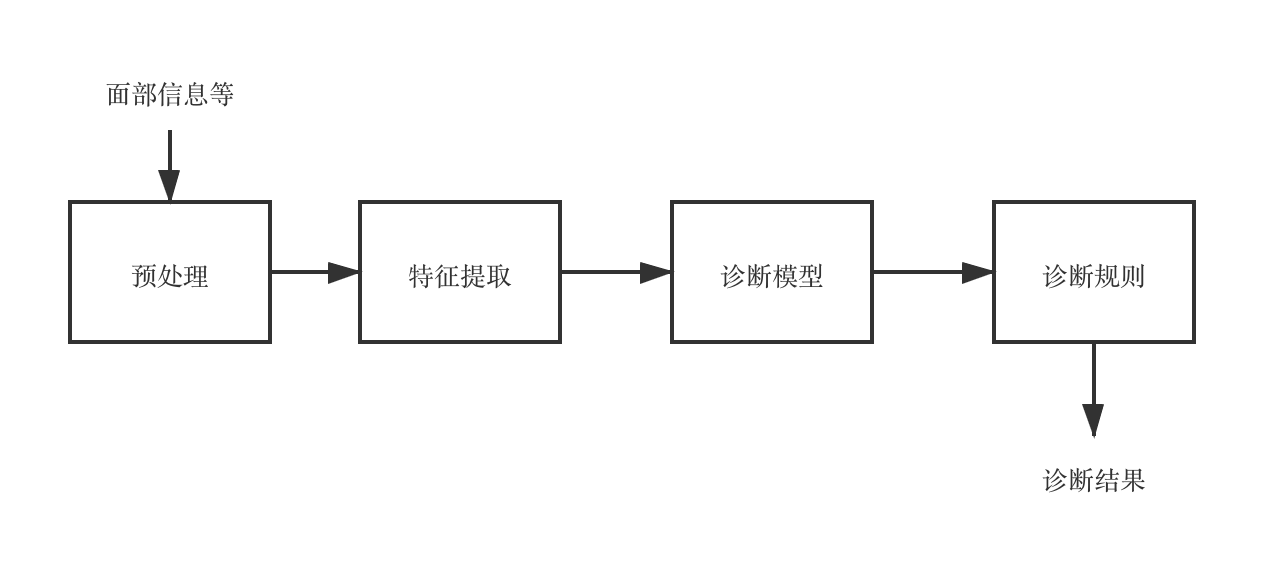
\includegraphics[width=12cm]{images/face777.png}
    \caption{面诊算法框架}
    \label{fig:face7778s}
\end{figure}

根据以上调研总结出面诊算法框架如\ref{fig:face7778s}所示,用户的面部信息作为基础输入,通过诊断模型将预处理和特征提取的结果转化为诊断结果,经过诊断规则可修正最终结果。
总的来说,面诊算法有以下特点:

\begin{itemize}
    \item 涉及的算法数量多,且随着技术的快速发展,算法更新迭代频率高。
    \item 不同的算法和算法之间有依赖关系。如面色分类算法,通常需要面部图片先经过色彩矫正、面部区域分割之后的图片作为输入。
    \item 诊断规则的加入能够提高整体诊断效果。
\end{itemize}

\subsubsection{面诊系统设计}

面诊作为诊断的一部分,医疗环境下的面诊系统很早便有人开始研究。
在医疗健康领域的标准环境下,面诊技术主要帮助提高医护人员工作效率,如辅助采集面部特征\cite{张红凯2015中医面诊信息采集与识别方法研究进展}、远程健康监控\cite{Hossain2015Cloud},面诊仪\cite{邸丹2016手持式舌象仪的研制}等。
这类技术特点主要有两点:
\begin{itemize}
    \item \textbf{为专业的医护人员设计}。医护人员有丰富的专业知识,有足够的时间学习系统如何使用。用户在使用的时候,有专业的医护人员指导或者解释最终的结果。
    \item \textbf{在诊所的标准环境下使用}。与日常健康场景相比,通常诊所环境使用的都是价格昂贵的标准的设备来保证系统的可靠性,而设备的体积与便携性通常不在考虑范围之内。
\end{itemize}


和标准环境下的面诊系统相比,日常健康场景用户多是在开放环境下使用。开放环境下的面诊系统更加容易受到光线、设备等因素的限制,因此对系统的准确性要求也相对较低,现有的面诊系统并不适合用户在日常场景下使用。此外,考虑到面诊算法数量多,迭代快的特点,如何有效地整合以及迭代这些面诊算法也是一个挑战。
总的来说,如何根据面诊技术的特点,设计出适合在日常场景下使用的面诊系统还是一个亟待解决的问题。

\subsection{人机交互领域中的日常健康技术}
人机交互关注以人为中心的系统设计,特别是关注慢性病患者与残疾人群体的日常使用体验。
以慢性病为例,大部分慢性病终身无法彻底治愈,因此多数慢性病患者会离开诊所环境回家自我调理。
慢性病患者需要日常生活中长期保持良好的健康习惯或坚持长期服药,因此一个好的日常健康管理系统对他们来说非常重要。

实际上,日常健康在人机交互研究中一直是热门的话题。
目前有大量研究关于各种类型的慢性病长期管理与追踪技术,以帮助慢性病患者和医护人员了解患者的健康状态并控制病情,
如糖尿病管理应用帮助用户记录血糖控制饮食\cite{burgermaster2019personal},精神患者通过远程监控应用及时提醒和帮助病情评估\cite{lazar2016evaluation}等。
此外,对于亚健康人员来说,健康行为引导技术可以帮助用户养成良好的健康习惯,指导更加健康的生活,
如通过记录饮食和运动习惯,或者通过额外的智能硬件设备记录呼吸、血压、心率等指标\cite{kay2012lullaby,gronvall2013beyond},让用户得到自身健康情况的反馈等。

目前人机交互中的健康追踪和行为引导技术,虽有大量关于日常健康场景下健康管理系统的交互设计研究,
但是目前只集中在慢性病管理以及利用呼吸、血压、心率、体重等特征,没有考虑到面部特征以及如何使用面诊技术进行日常健康管理。

综合上述的相关工作和背景介绍,可以总结出本文的主要研究挑战分为以下三点:

\begin{enumerate}
    \item \textbf{对日常健康场景下面诊系统的技术特点与用户行为模式分析。}
    一方面,目前已有的面诊系统设计,缺乏对日常健康场景下的研究;
    另一方面,人机交互领域虽然有大量关于日常健康管理的研究,但没有考虑到面诊技术的特点设计面诊系统。
    在日常健康场景下,面诊系统的技术特点,用户的交互行为和心理模式都是未知的。

    \item \textbf{日常健康场景下面诊系统的设计策略。}
    如挑战1所述,目前关于日常健康场景下面诊系统的设计策略还是空白的。
    关于指导日常场景下面诊系统如何设计的问题,需要结合目前人机交互中已有的设计策略以及挑战1的研究结论进行深入讨论。

    \item \textbf{日常健康场景下面诊系统的设计及实现。}
    挑战2提到的设计策略可以指导面诊系统的设计与实现。
    如何在设计策略的基础上,结合目前已有的面诊系统系统设计与人机交互设计,设计并具体实现适合日常健康场景的面诊系统仍待解决。
    
\end{enumerate}

\section{本文研究内容与创新}

本文以日常健康场景下面诊技术的应用问题,使用基于人机交互的研究方法,最终实现了一个面向日常场景场景的面诊系统,主要工作如下:

\subsection{面向日常健康的面诊系统设计方法}

目前大部分的面诊技术主要应用场景在诊所环境下,没有考虑到日常场景下系统如何设计;
而人机交互虽有大量关于日常场景下的健康管理工作,但都集中在慢性病管理以及基于心率、血压、体重等信息进行系统设计,没有探索如何使用面部信息以及研究面部信息在使用中的特点。

为解决日常场景下面诊系统的设计问题,本文基于技术探针的设计方法做了以下工作:
本文实现了一个名为云中医应用的技术探针并开展实验,探索了日常健康场景下面诊技术的特点以及待解决的问题,并提出了对应的日常健康场景下如何设计面诊应用的设计策略,
填补了日常健康场景下面诊技术的应用研究的空白\cite{ding2019reading}。

通过用户研究和数据分析本文发现,和诊所环境相比,日常健康场景下基于面诊技术的健康管理应用主要有以下几点问题亟待解决: 

\begin{itemize}
    
    \item \textbf{长期使用问题}。诊所环境下,面诊技术默认只考虑用户在就诊时的单次使用。日常健康场景下的面诊技术应用,需要考虑用户多次使用并且跟踪用户的使用情况,是一个长期的过程。在日常健康场景下,如何吸引用户继续使用、如果提高日常使用场景下交互的便捷性、如何引导用户改变自己的生活方式,提高生活质量等也是需要考虑的问题。
    
    \item \textbf{日常可用性问题}。日常场景下面诊系统的特殊点在于,用户在使用过程中需要拍面部或者舌头。在中国当前比较传统的文化背景下,大部人在公共场合伸出舌头会感觉比较尴尬或者感觉不雅观影响个人形象。

    \item \textbf{设备的多样性问题}。在诊所环境下,用户是在专门的设备下进行健康诊断。而在日常健康场景下,所有操作都在用户的移动设备上完成。用户的移动设备差异性比较大,特别是安卓系统的碎片化问题非常严重。不同用户的设备从移动操作系统到硬件计算能力和存储空间的都存在很大的差异性。如何在不同的用户设备环境下,让用户快速稳定地完成面诊流程是一个待解决的问题。
    
    \item \textbf{用户的多样性问题}。各类用户的受教育程度,日常空余时间,职业、工作场合是需要考虑的因素。比如在日常使用的时候,与诊所环境下不同,用户在使用过程中可询问的专业技术人员,大部分用户没有医疗相关的专业知识,使用起来会比较困难,在日常健康场景下帮助用户理解诊断过程和诊断结果难度更大。
    
    \item \textbf{敏感性问题}。用户在日常健康场景下完成面诊的过程中,可能会因为需要拍面部、伸出舌头拍舌苔而感到尴尬,限制了用户的日常使用范围。
    
    \item \textbf{信赖问题}。在面诊系统由权威的诊所迁移到日常场景后,许多用户对系统的结果持怀疑态度,从而导致他们不信赖系统。在没有其他的评估机制验证结果有效性的前提下,也会让用户对系统产生怀疑。
    
    \item \textbf{情绪问题}。直白地展示诊断结果,特别是系统给出负面结果时,会让用户产生明显的消极情绪并放弃继续使用。 

\end{itemize}

针对这些问题,本文分别提出了以下几点设计策略:
\begin{itemize}
    \item \textbf{支持可持续使用}。针对长期使用问题,本文在交互和系统设计上提出了对应的解决思路。在交互上,对于健康状况有变化的用户,允许用户跳过某些步骤,突出显示变化的部分;对于健康状况没有变化的用户,加入上下文信息如天气、时令等信息,增加用户的新鲜感。在系统设计上,根据用户的反馈,增加健康知识推送能够增加系统的可变性,吸引用户持续使用。
    \item \textbf{系统可解释性}。针对信赖问题,本文提出了可解释的系统设计:暴露系统的技术原理和开发背景,提高可信度;解释系统的局限性,帮助用户理解系统。此外,在后续的系统实现中,本文对诊断任务进行建模,通过拆分诊断过程,暴露每个中间过程的结果,以实现诊断结果的可解释性。
    \item \textbf{日常可用性}。针对长期使用和日常可用性问题,本文提出将诊断步骤设置为可选项,并且记录用户的历史信息以达到避免使用尴尬和操作繁琐的问题。
\end{itemize}


\subsection{面向日常健康的面诊系统的设计与实现}
一方面,通过调研市面上主流的面诊系统,本文发现目前大多面诊系统都非常地定制化,依赖特定的设备和模型,没有一个统一的面诊系统设计方案;
另一方面,为了解决前期研究发现的用户在日常健康场景使用遇到的各种问题,同时解决当前面诊系统没有统一的模型管理等缺点,本文对面诊系统进行了抽象建模,基于图的方法管理模型,实现了一个适用于日常健康场景的可扩展的面诊系统。
本文在系统设计层面做了以下几点工作,其中1-3为系统设计方面,4为交互设计方面:

\begin{itemize}

    \item 跨平台实现与模型服务化。为了解决日常场景下\textbf{用户设备多样性}带来的各种使用上的问题,本文采用了跨平台方案与容器化方法,让模型在服务端运行,屏蔽了用户的设备差异。
    为了解决\textbf{系统的稳定性与性能问题},通过容器化方法将算法模型打包成独立的服务,并实现了简单的分布式主从模块。

    \item 诊断任务拆分与管理。为了解决\textbf{系统可解释性问题},本文对诊断任务进行了拆分。一次完整诊断任务包含预处理、特征提取与特征分类等子任务。对诊断任务进行拆分,可以提高系统资源利用率和灵活性。
    同时,通过对诊断任务拆分,每个子任务暴露出来的中间结果,为面向日常健康场景的交互设计提供可解释的基础。
    现有的可解释工作,主要依赖可解释的交互元素,自解释的模型如卷积和attention机制等\cite{abdul2018trends},在当前众多面诊模型中不具有通用性。
    因此本文结合面诊技术流程长,涉及算法多等特点,使用任务拆分方式,在系统设计层面提供了面诊过程的可解释性设计。
    
    \item 基于有向无环图的模型管理。为了解决\textbf{面诊算法更新迭代快}带来的问题,本文对一次面诊过程进行了建模,将用户信息输入到诊断结果中的模型依赖抽象为一个大的有向无环图,将诊断规则定义为合并节点,方便后续增加模型实例数与模型迭代,同时避免了多个输出节点的问题。
    
    \item 面向日常健康场景的交互设计。为了解决用户日常场景下的\textbf{长期使用、实用性、敏感性、情绪与信赖等问题},本文提出了并实现了可解释、日常可用的交互设计。

\end{itemize}

最后,本文基于系统设计,实现了更加适合日常健康场景下使用的面诊系统,并通过实验进行了验证。

\section{本文研究方法}

% 定性研究, 强调context的重要性,以人为中心,重视用户的体验。
人机交互(Human-Computer Interaction)指的是用户与可交互的计算机系统(包括传统计算机与各类智能设备)之间的交互设计与实现,其研究强调上下文的重要性,涵盖了计算机科学、社会学、心理学等学科,重视技术如何更好地为人服务\cite{lazar2017research}。
在探索以人为中心的相关交互设计、系统设计方面,人机交互研究也有相关的方法论以及数据获取方法\cite{lazar2017research}。
本小节将简单介绍本文所使用的研究方法及其数据获取方法。

% 为什么要用技术探针
通常,典型的人机交互研究中研究系统设计是访问用户的家庭,然后设计并实现一个系统,让用户评价。
在日常健康场景下,这种设计方法缺点比较明显\cite{Hutchinson2003Technology}:

\begin{itemize}
    \item 没有激发用户的思考,可能无法反映用户的实际需求和掩盖在家庭内部之间``好玩''的设计。
    \item 在设计和实现系统过程中,没有提供真实的长期使用场景,用户缺乏参与性。
\end{itemize}


% 介绍什么是技术探针
为了避免上述的问题,Hutchinson等\cite{Hutchinson2003Technology}提出了一种名为技术探针的研究方法:利用快速开发出来的、功能并不完善的简单系统,让用户在实际使用探针的过程中,鼓励用户大声表达自己异想天开的想法,在草稿上画出自己心中的系统,参与设计过程。
基于技术探针的方法主要用于系统设计的早期阶段\cite{turmo2020training},也经常被用来为日常使用的健康技术的设计提供信息。
目前已有不少成功使用案例,例如通过技术探针的设计方法,Papi等人\cite{papi2015knee}利用可穿戴式膝关节原型,探索了在家庭环境下如何设计用于骨关节炎患者的康复工具;同样,Singh等人\cite{singh2017supporting}通过1-2周的用户研究,利用技术探针,研究了如何设计慢性疼痛患者使用的日常可穿戴设备。

在计算机领域,常见的用户数据获取是通过大量统计数据,如大批量结构化的问卷、用户行为日志等,然后在分析过程中,通过提取自变量、因变量做变量的相关性分析得到最终的结论。
在人机交互研究中,通常采用获取数据的方法是通过资料分析、案例分析、直接观察、用户访谈等方式获取研究数据。
其中,深度访谈是交互研究领域中收集数据最常用的一种方式,通过开放式、半结构化的面对面访谈,能够深度了解调查者内心的客观想法,避免研究者的主观判断。
该方法在心理学与社会学领域被广泛应用,能够发掘出用户更细节的需求和想法。
同时,在挑选了足够的代表性采访对象的前提下,该方法相对地对数据量的要求不高,在连续访谈得到的结果比较稳定后就可以停止访谈\cite{cleary2014data}。
本文使用两者相结合的方式:在使用技术探针进行实验之后,首先通过分析日志和问卷,得到大致的结论,然后通过面对面深度访谈发掘更深层次的原因,得到最终的结论。

% 技术探针, 文化探针 等


\section{论文结构}
本文按照一共组织了六个章节,具体的论文结构如下:

第一章,绪论。介绍了本文工作的研究背景和研究意义,概括了当前的研究现状和存在的问题,最后介绍了本文的主要工作和创新点。

第二章,相关工作。介绍了当前比较流行的基于面诊技术的应用,并描述了当前人机交互中相关日常健康场景的研究重点。

第三章,基于技术探针的设计方法。就本文的研究问题,采用技术探针的方法进行了探索了日常健康场景下面诊系统应该如何设计。设计了调研问卷和深度访谈。通过对访谈数据的仔细分析,总结出了日常健康场景下面诊技术的特点,发现了其中存在的问题。

第四章,面向日常健康的面诊系统设计。为解决当前面诊系统在日常健康场景中存在的诸多问题,本文提出了面向日常健康场景的面诊系统设计并进行了实现。

第五章,验证实验。本文对面向日常健康场景的面诊系统进行了性能测试,并通过验证实验,验证了交互设计工作的有效性。

第六章,总结与展望。总结了本文的三个主要工作内容和不足之处,并对后续工作进行了展望。